
\chapter{Binary Tree}
\label{cha:binary-tree}

A \keyword{tree} is a frequently-used data structure to simulate a hierarchical tree structure.
Each node of the tree will have a \keyword{root} value and a list of references to other nodes which are called \keyword{child} nodes.



A \keyword{Binary Tree} is one of the most typical tree structure.
As the name suggests, a binary tree is a tree data structure in which each node has at most two children, which are referred to as the \keyword{left} child and the \keyword{right} child, as shown in Figure \ref{fig:binary-tree}.
\begin{figure}[!ht]
  \centering
  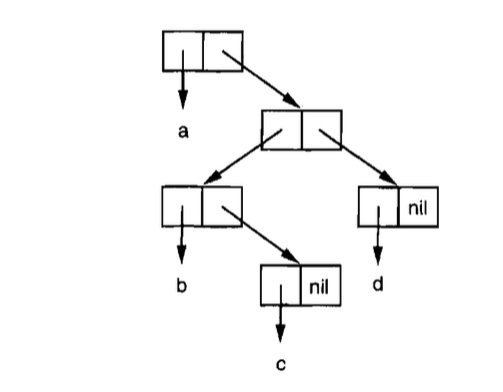
\includegraphics[width=0.6\textwidth]{binary-tree.png}
  \caption{Binary tree}
  \label{fig:binary-tree}
\end{figure}






\section{Traverse a Tree}
\label{sec:traverse-tree}

There are 4 common used traversal:
\begin{itemize}
\item Pre-order Traversal
\item In-order Traversal
\item Post-order Traversal
\item Level-order Traversal
\end{itemize}


The pre-in-post order references the \keyword{root}.

Pre-order traversal is to visit the \keyword{root} first.
Then traverse the left subtree.
Finally, traverse the right subtree.

In-order traversal is to traverse the left subtree first.
Then visit the \keyword{root}.
Finally, traverse the right subtree.

Post-order traversal is to traverse the left subtree first.
Then traverse the right subtree.
Finally, visit the \keyword{root}.

Level-order traversal is to traverse the nodes by level from root to leaves.
In the same level, traverse from left to right.

Take the Figure \ref{fig:binary-tree} for example.
Pre-order traversal generate the sequence: \([8\ 3\ 1\ 6\ 4\ 7\ 10\ 14\ 13]\).
In-order traversal generate the sequence: \([1\ 3\ 4\ 6\ 7\ 8\ 10\ 13\ 14]\).
Post-order traversal generate the sequence: \([1\ 4\ 7\ 6\ 3\ 13\ 14\ 10\ 8]\).
Level-order traversal generate the sequence: \([8\ 3\ 10\ 1\ 6\ 14\ 4\ 7\ 13]\).


\section{Examples}
\label{sec:examples-1}

Here are some codes about binary tree on \href{https://github.com/mingmingli916/algorithms/tree/main/binary_tree}{Github}.

%%% Local Variables:
%%% mode: latex
%%% TeX-master: "algorithms"
%%% End:
